%========================%
%        Preamble        %
%========================%
\documentclass[12pt]{amsart}

    %========================%
%        Packages        %
%========================%

\usepackage[utf8]{inputenc}
%\usepackage{amsmath}    % Included in amsart package
%\usepackage{amsthm}     % 
\usepackage{amssymb}      % 
\usepackage{mathtools}      % Paired Limiter Macros
% \usepackage{mdframed}       % boxes for theorem
\usepackage{enumitem}     % Continuous numbering of lists
\usepackage[hidelinks]{hyperref}
\usepackage{tikz}
\usetikzlibrary{positioning}
\usepackage{blindtext}
\usepackage{graphicx}
\usepackage{float}

%========================% 
%          Title         %
%========================% 
\title{Chapters 21 and 22 Notes}
\author{Anish Sundaram}
\date{\today}

%========================% 
%        Theorems        %
%========================% 
\theoremstyle{definition}
\newtheorem{theorem}{Theorem}  % Boxed theorems
\newtheorem{definition}{Definition} % Definitions
\newtheorem{example}{Example}       %
\newtheorem{algorithm}{Algorithm}
\newtheorem*{proof*}{Proof}         % non-numbered
\newtheorem*{remark}{Remark}        %
\numberwithin{equation}{theorem}    % Local equation numbering

\setcounter{tocdepth}{3}      % Show subsubsections in contents

%========================% 
%        Macros          %
%========================% 
\DeclarePairedDelimiter\abs{\lvert}{\rvert}  % Vertical bars
\DeclarePairedDelimiter\norm{\lVert}{\rVert} % Double vertical bars
\newcommand{\drawvec}[1]{                    % matrices on one line
    \begin{bmatrix}
        #1
    \end{bmatrix}
}


% \begin{figure}[H]
%     \centering
%     \includegraphics[width=5in]{global-carbon-cycle.png}
%     \caption{The Global Carbon Cycle}
%     \label{global-carbon-cycle}
% \end{figure}

%========================% 
%         Document       %
%========================% 
\begin{document}

\maketitle

\tableofcontents

\section*{21. Electric Charge and Electric Field}
Electromagnetic interactions involve particles that have electric charge, 
an attribute that is as fundamental as mass. Just as objects with mass are 
accelerated by gravitational forces, so electrically charged objects are 
accelerated by electric forces.


\subsection*{21.1 Electric Charge}
\begin{definition}
    \textbf{Electric Charge}: 
    is the state of having more or less than a natural
    amount of electrons.\textit{Positive} if less or \textit{Negative} if more. 
    \begin{remark}
        Two positive charges or two negative charges repel each other. A 
        positive charge and a negative charge attract each other.
    \end{remark}
\end{definition}

\begin{definition}
    \textbf{Electrostatics}: 
    the interactions between electric charges that are 
    at rest (or nearly so).
\end{definition}

\subsubsection*{21.1.1 Electric Charge and the Structure of Matter}

\begin{definition}
    \textbf{Parts of Atom}: 
    Positive Protons, negative Electrons and Neutral 
    Neutrons. Protons and Neutrons are held by \textit{Strong Nuclear Force} 
    to form the Nucleus and are themselves comprised of \textit{Quarks}. 
    The Majority of Atom is the \textit{Electron Cloud}
\end{definition}

\begin{definition}
    \textbf{Ionization}: 
    Normally positive charge and negative charge cancel 
    out, but through an addition or loss of an electron the atom becomes 
    ionized, becoming either a \textit{positive} or \textit{negative} ion 
\end{definition}

\begin{figure}[H]
    \centering
    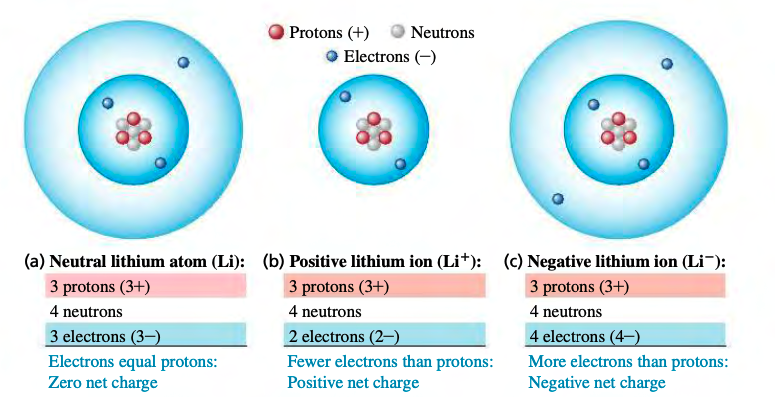
\includegraphics[width=5in]{Media/Atomic.png}
    \caption{Atomic Structure and Ionization}
    \label{Atomic Structure and Ionization}
\end{figure}

\subsubsection*{21.1.2 Electric Charge is Conserved}

\begin{theorem}
    \underline{Principle of conservation of charge}:
    The algebraic sum of all the electric charges in any closed system is 
    constant. In any charging process, charge is not created or destroyed; 
    it is merely transferred from one body to another.
\end{theorem}

\begin{theorem}
    \underline{Quantized Nature of Charge}:
    The magnitude of charge of the electron or proton is a natural unit of charge.
\end{theorem}

\subsection*{21.2 Conductors, Insulators, and Induced Charges}
\begin{definition}
    \textbf{Conductivity and Insulation}: 
    \textit{Conductors} are materials that transfer electrons well, such as 
    copper and other metals. The opposite are \textit{Insulators} which are 
    poor and transfering charge, these are often nonmetals. Some materials 
    called \textit{semiconductors} are intermediate in their properties between
    good conductors and good insulators.
\end{definition}

\subsubsection*{21.2.1 Charging by Induction}

\begin{definition}
    \textbf{Induction}: 
    a method used to charge an object without actually touching the object to 
    any other charged object. This is done by rearranging electrons already 
    present in object
\end{definition}

\begin{definition}
    \textbf{Polarization}: 
    The slight shifting of charge within the molecules of the neutral insulator
    when placed near a charge object. This is what causes charge by Induction
\end{definition}

\begin{figure}[H]
    \centering
    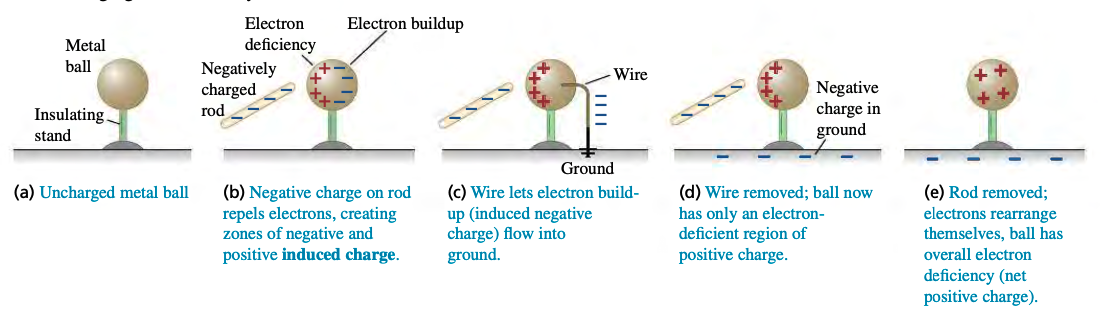
\includegraphics[width=5in]{Media/Induction.png}
    \caption{Charge by Induction}
    \label{Charge by Induction}
\end{figure}







\end{document}